\documentclass[a4paper,12pt]{article}
% if you need additional LaTeX packages, add them here
\usepackage[]{geometry}
\usepackage{graphicx, wrapfig, enumitem}
\usepackage{subcaption}
\usepackage{xcolor}
\usepackage{listings, ulem}
\usepackage[most]{tcolorbox}
\usepackage{multirow, multicol, tabularx, booktabs}
\usepackage{fancyhdr}
\usepackage{tikz}
\usepackage{hyperref}
\usepackage[simplified]{pgf-umlcd}
\usepackage{subfiles}
\usepackage[linguistics]{forest}
\usepackage{caption}
\usepackage{circuitikz}

\graphicspath{{Resources/}}

\setlist{nolistsep}
\setlength{\parindent}{0in}


\usetikzlibrary{decorations.markings}
\usetikzlibrary{calc}
\tikzset{middlearrow/.style={
        decoration={markings,
            mark= at position 0.5 with {\arrow{#1}} ,
        },
        postaction={decorate}
    }
}
\def\centerarc[#1](#2)(#3:#4:#5)% Syntax: [draw options] (center) (initial angle:final angle:radius)
    { \draw[#1] ($(#2)+({#5*cos(#3)},{#5*sin(#3)})$) arc (#3:#4:#5); }


\newcommand\ilkeFonts{
    \usepackage{fontspec}
    \setmainfont{texgyrepagella-regular.otf}[
        BoldFont       = texgyrepagella-bold.otf,
        ItalicFont     = texgyrepagella-italic.otf,
        BoldItalicFont = texgyrepagella-bolditalic.otf,
        Scale = MatchLowercase
    ]
                    
    \setmonofont{Inconsolatazi4-Regular.otf}[
        BoldFont  = Inconsolatazi4-Bold.otf, 
        Scale     = MatchLowercase
    ]
    
    \setsansfont{MerriweatherSans-Regular.ttf}[
        BoldFont       = MerriweatherSans-ExtraBold.ttf,
        ItalicFont     = MerriweatherSans-Italic.ttf,
        BoldItalicFont = MerriweatherSans-ExBoldIt.ttf,
        Scale = MatchLowercase
    ]
}
\ifxetex%
    \ilkeFonts%
\else\ifluatex%
    \ilkeFonts%
\else%
    % \usepackage[sc]{mathpazo} % Palatino-like serif font
    \usepackage[T1]{fontenc}
    \usepackage[scaled=1]{inconsolata} % Fixed-width font
    \usepackage[sf]{merriweather}
\fi

\hypersetup{colorlinks=true, linkcolor=blue!50!red, urlcolor=green!70!black}


\pagestyle{fancy}
\fancyfoot[L,C,R]{}
\fancyhead[L,C,R]{}
\fancyfoot[L]{}
% \fancyfoot[R]{\thepage}
\fancyhead[R]{TinyBot : \thepage}
\fancyhead[L]{
    
\includegraphics[height=1cm]{CRoCLogo(mediumquality).png}
    % 
\includegraphics{Resources/CRoCLogo(mediumquality).png}
}


\title{	
    \begin{center}
        
\includegraphics[width=0.15\textwidth]{CRoCLogo(mediumquality).png}
    \end{center}
	\normalfont\normalsize
	\textsc{Curtin Robotics Club}\\ % Your university, school and/or department name(s)
	\vspace{25pt} % Whitespace
	\rule{\linewidth}{0.5pt}\\ % Thin top horizontal rule
	\vspace{20pt} % Whitespace
    {\huge TinyBot }\\
    % {\huge Assignment Report}\\ % The assignment title
	\vspace{12pt} % Whitespace
	\rule{\linewidth}{2pt}\\ % Thick bottom horizontal rule
	\vspace{12pt} % Whitespace
}

\author{\LARGE Ilke Dincer \\ \small ilke@curtinrobotics.org} % Your name

\date{\normalsize\today} % Today's date (\today) or a custom date

\begin{document}

\pagenumbering{gobble}
\maketitle

\pagebreak
\pagenumbering{roman}
\tableofcontents

\pagebreak
\pagenumbering{arabic}

\section{Introduction}

There are many different components of a robot; the most important being the microcontroller (the brain), the motors (the legs), and any sensors (how the robot sees the world).

This guide will take you through building a simple robot dubbed TinyBot. It has 2 wheels, a caster wheel, a battery, an arduino, and a breadboard.


\section{Components}
 
\begin{tabularx}{\linewidth}{cccX}
    \toprule
    Component & Quantity & Price & Sources \\ \midrule
    Arduino Uno & 1 & \$5-\$80 & Arduino's are discuessed in Section \ref{sec:microcontroller}. A genuine Arduino will cost about \$80, however Arduino clones can be bought online for as little as \$5. Ebay is a good starting point for finding an Uno. \\
    Breadboard & 1 & & \\
    N20 Motor & 2 & & \\
    H-Bridge & 1 & & \\  
    Wheels & 2& \$0 & The wheels for this project are 3D printed, and are supplied by the club. \\
    Caster Wheel & 1 & ? & The caster wheel consists of 2 parts, a marble and it's 3D printed casing. The 3D print will be supplied by the club at no charge, however you must source your own marble.\\
    \bottomrule
\end{tabularx}

\bigskip

Additional sensors can be bought and integrated with TinyBot, however that is not covered in this project guide. 

\section{Construction}

\pagebreak
\section{Microcontroller} \label{sec:microcontroller}
\begin{wrapfigure}{l}{0.2\textwidth}
    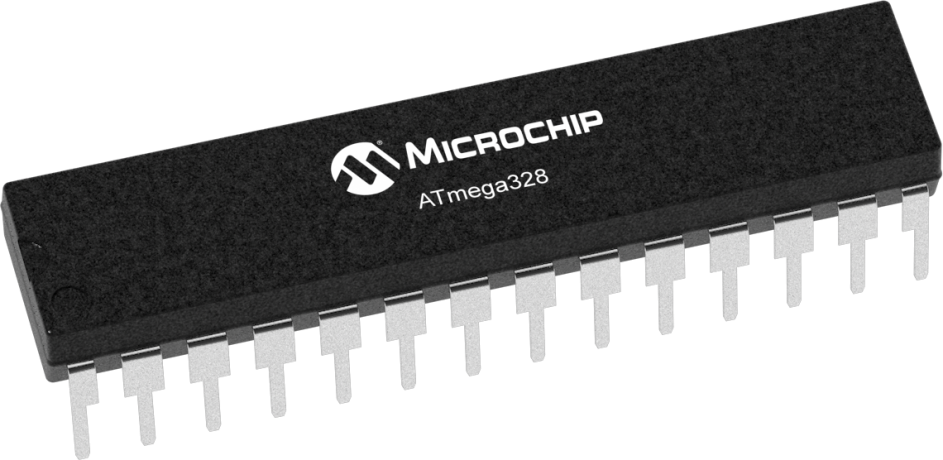
\includegraphics[width=0.18\textwidth]{medium-ATmega328-SPDIP-28.png}
    \captionof{figure}{A Microchip}
    \label{fig:microchip}
\end{wrapfigure}

A microcontroller is a really small microcomputer on a very small chip, see Figure \ref{fig:microchip}.
These are used in a variety of devices; including robots, vending machines, phones, computers, etc. \\

Arduino's are a development board; consisting of an microcontroller, power regulation, and input/output (also known as IO) pins. As microcontrollers are very tiny prototyping with them or using them to build something would be really difficult. The purpose of an arduino is to provide a medium that allows easy development with microcontrollers. There are many different kinds of arduinos, each using a different microchip.  \\

\begin{wrapfigure}[12]{r}{0.3\textwidth}
    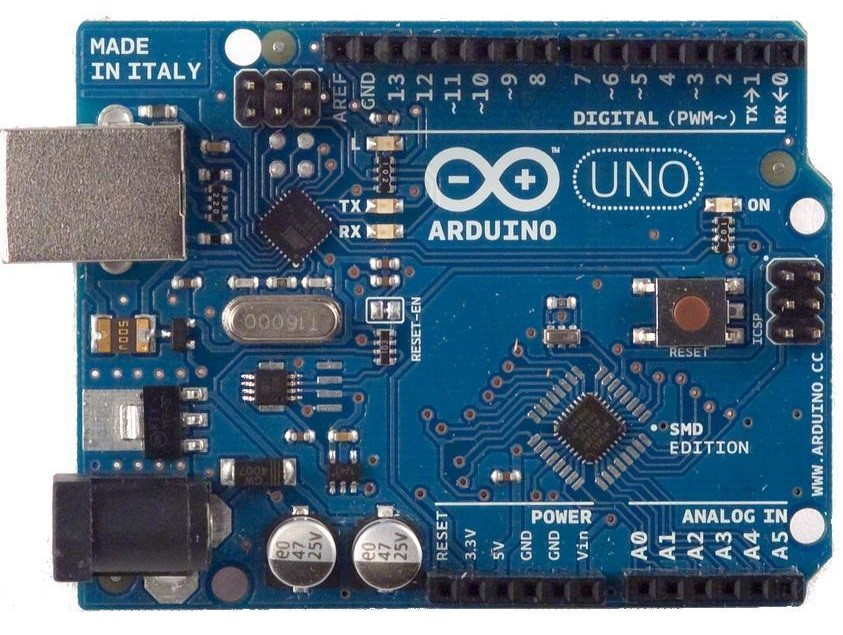
\includegraphics[width=0.3\textwidth]{arduino-uno.jpg}
    \caption{An Arduino Uno}
    \label{fig:arduino-real}
\end{wrapfigure}


The Arduino used in this project is the Arduino Uno, which has an ATMega328p microchip as shown in Figure \ref{fig:microchip}. Figure \ref{fig:arduino-real} is what a real Arduino Uno looks like, though the colour and text may be different from brand to brand. Genuine Arduinos are quite expensive, and there are many clones available which are much cheaper. Figure \ref{fig:arduino-pinout} shows a stylised view of an Uno, labelling all the different pinouts. \\

Arduino's and other development boards are used extensively by hobbyists, they are cheap, easy to use, and extremely versatile. Arduino's are used in nearly every project that CRoC runs, and so are very useful to learn to use. 


\begin{center}
    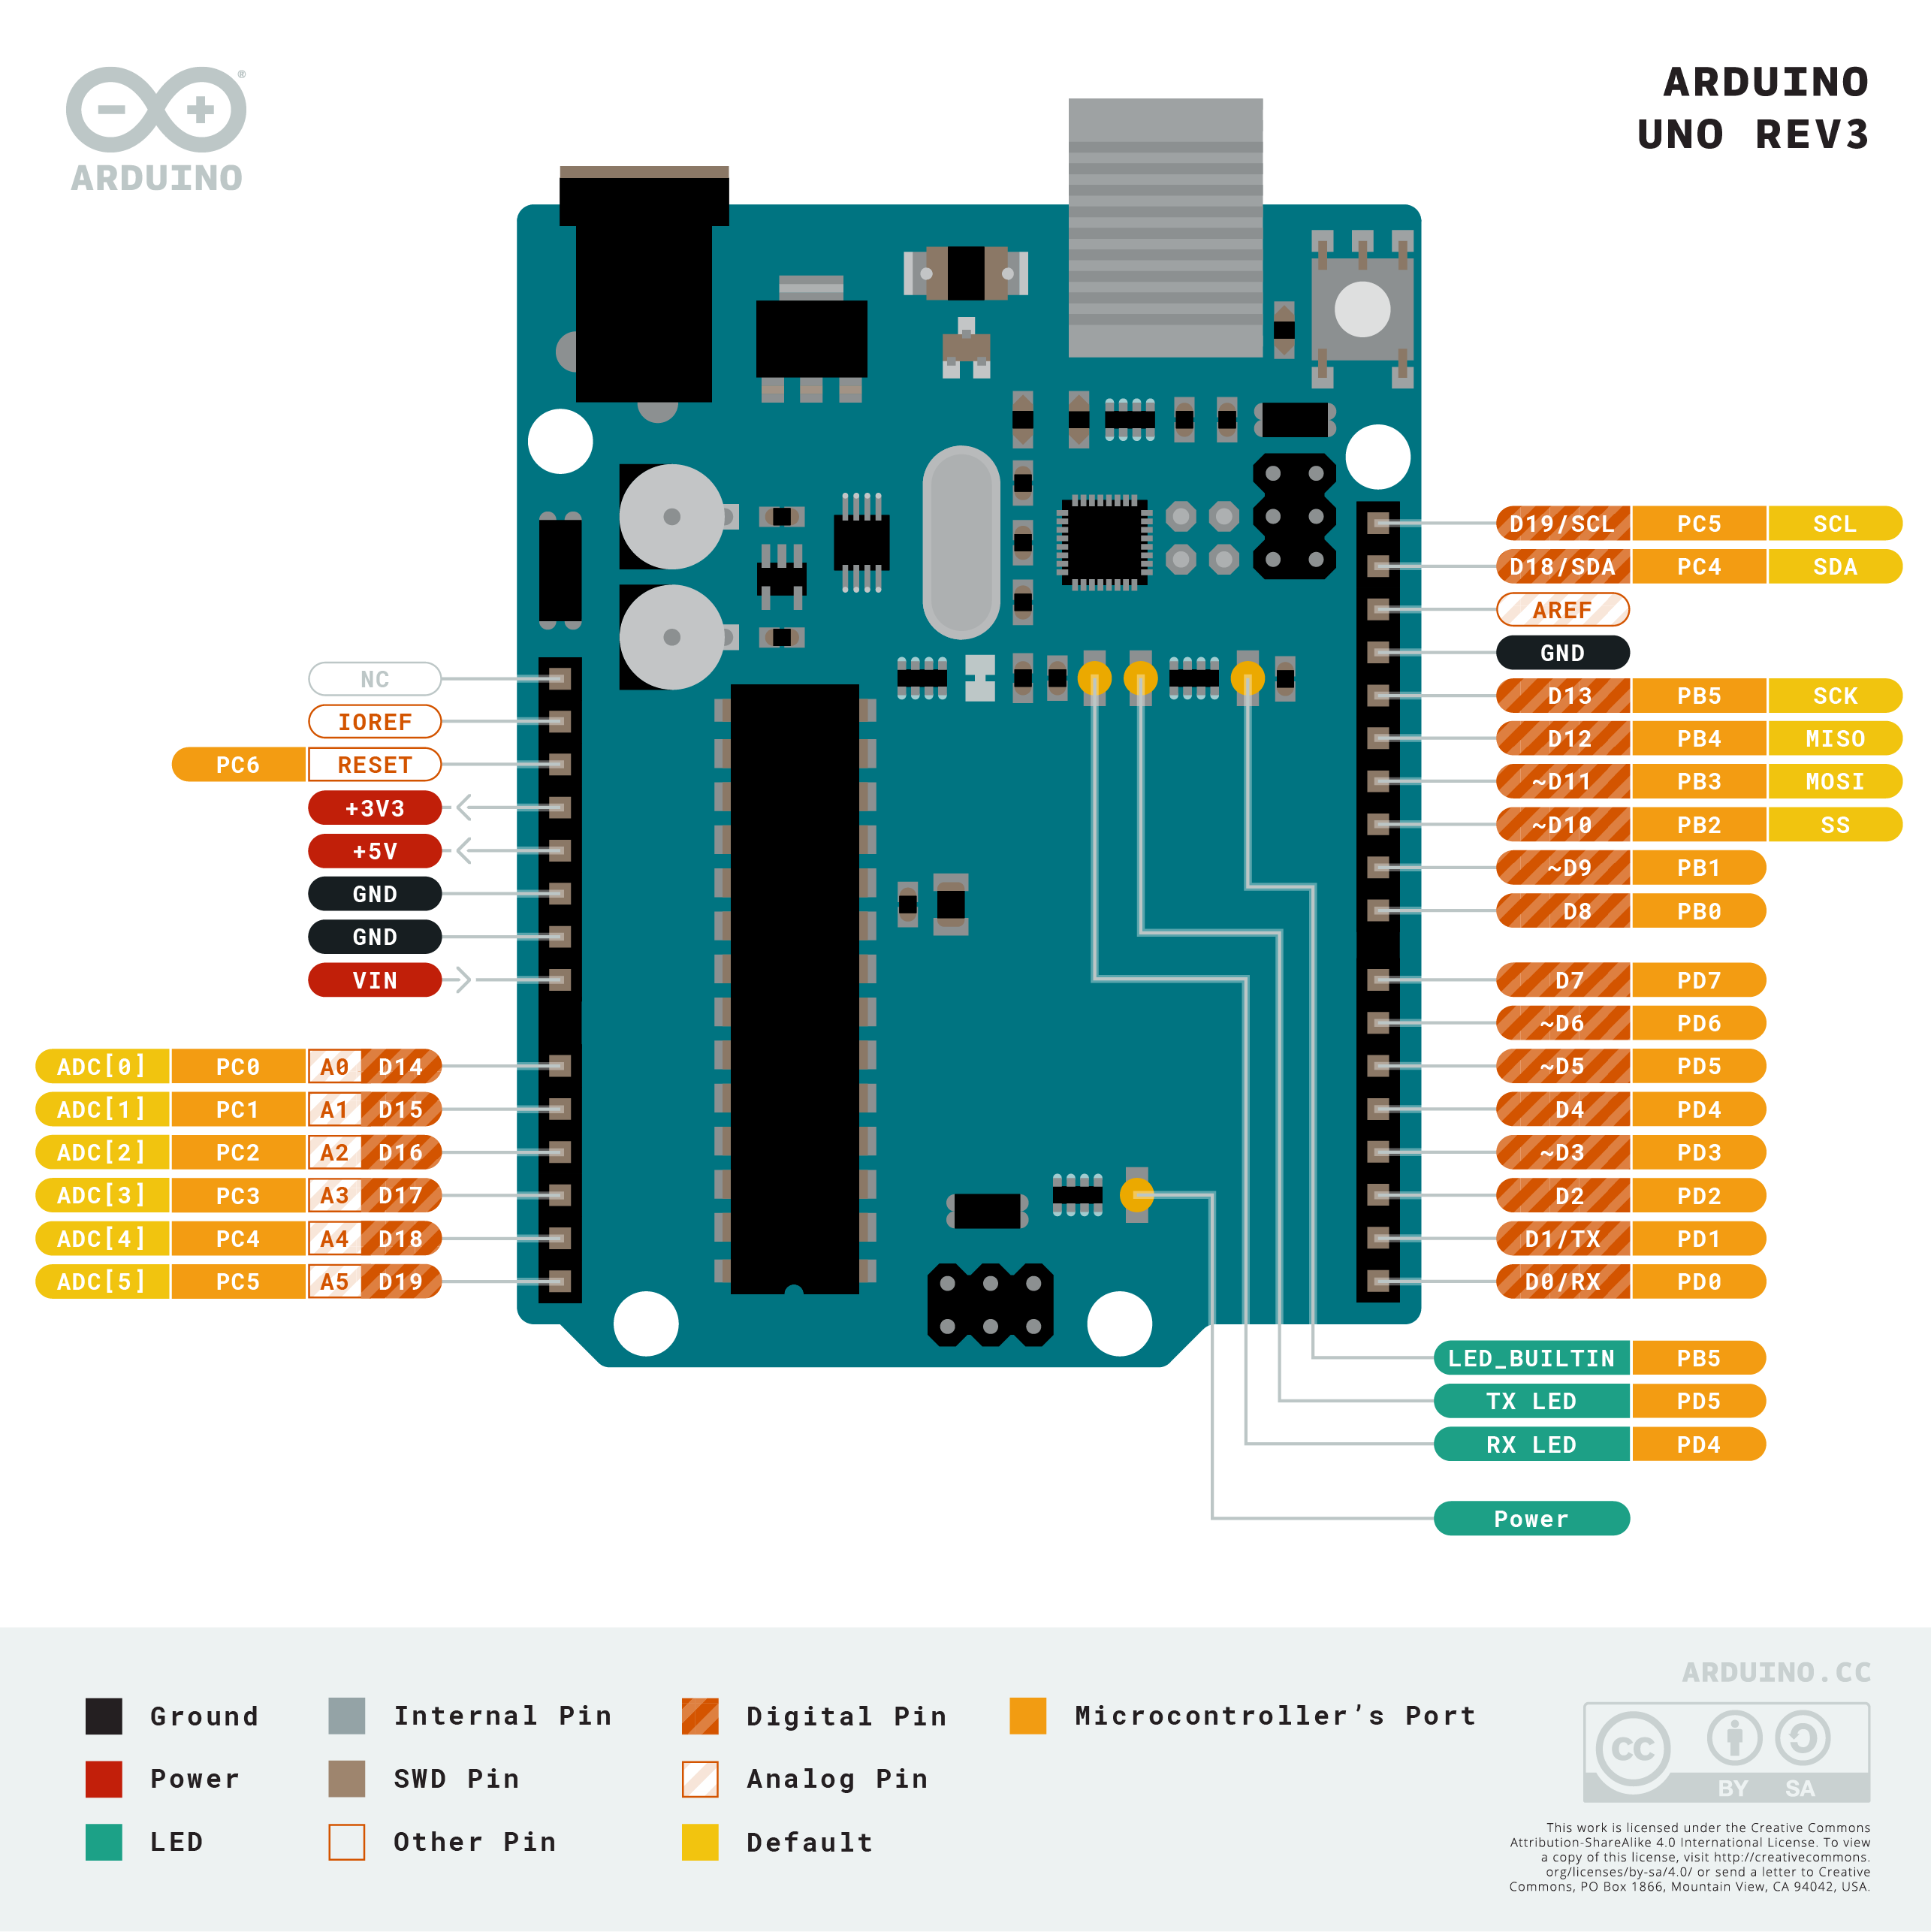
\includegraphics[width=0.8\linewidth]{Pinout-UNOrev3_latest.png}
    \captionof{figure}{Pinout of Arduino Uno}
    \label{fig:arduino-pinout}
\end{center}





\section{Motor}
gearbox, motor

\pagebreak
\section{Motor Controller}

The simplest way to drive a motor is to run a current through the motor. This will make the motor run in one direction, though it is impossible to control the speed, direction, or to stop the motor. \\

A simple solution to this is to use a h-bridge. The simplest h-bridge is shown below, the voltage source is on the left and ground on the right. 


\begin{center}
    
    \begin{circuitikz}
    \draw (0,2) -- (0,0) to
        (0,0) to[nos, l_=$1$] (2,0) to
        (2,0) to [nos, l_=$2$] (4,0) to
        (4,0) -- (4,2) to
        (4,2) to[nos, l_=$3$] (2,2) to
        (2,2) to[nos, l_=$4$] (0,2);
    \draw (2,1) node[elmech](motor){M};
    \draw (motor.north) -- (2,2);
    \draw (motor.south) -- (2,0);
    \draw (0,1) -- (-1,1) node[vee]{};
    \draw (4,1) -- (5,1) node[ground]{};
    % \draw (2,0) to[sV, color=white, name=M] (2,2);
    % \mymotor{M}{90};
    % \draw[rotate=2] (0,2) \mymotor{M}{90} (2,2);
    \end{circuitikz}
    % \captionof{figure}{}
\end{center}

When switches $1$ and $3$ are closed, the current will flow through the motor making it turn anticlockwise.
% in the motor will flow in one direction. 

\begin{center}
    \begin{circuitikz}
        \draw (0,2) -- (0,0) to
            % (0,0) to[o-o, l_=$1$] (2,0) to
            (0,0) -- node[below, yshift=-1.5mm]{1} (2,0) to
            (2,0) to [nos, l_=$2$] (4,0) to
            (4,0) -- (4,2) to
            % (4,2) to[l_=$3$] (2,2) to
            (4,2) -- node[above, yshift=1.5mm]{3} (2,2) to
            (2,2) to[nos, l_=$4$] (0,2);
        \draw (motor.north) -- (2,2);
        \draw (motor.south) -- (2,0);
        \draw[color=red!100, thick] (0,1) -- (-1,1) node[vee]{};
        \draw[color=red!100, thick] (4,1) -- (5,1) node[ground]{};
        
        % \draw[color=red!100] (0,2) -- (0,0) to
        % (0,0) -- (2,0) to
        % (2,0) -- (4,0) to
        % (4,0) -- (4,2) to
        % (4,2) -- (2,2) to
        % (2,2) -- (0,2);


        \begin{scope}[>=latex]
            \draw[->, color=red!100, thick] (-1,1) -- (0,1);
            \draw[->, color=red!100, thick] (0,1) -- (0,0);
            \draw[->, color=red!100, thick] (0,0) -- (2,0);
            \draw[->, color=red!100, thick] (2,0) -- (2,2);
            \draw[->, color=red!100, thick] (2,2) -- (4,2); 
            \draw[->, color=red!100, thick] (4,2) -- (4,1);
        \end{scope}
        \draw (2,1) node[elmech](motor){M};
        \centerarc[->](2,1)(-45:45:0.7);
        \centerarc[->](2,1)(135:225:0.7);
    \end{circuitikz}
\end{center}

In the same vein, closing switches 2 and 4 will cause the motor to turn clockwise. 
\begin{center}
    \begin{circuitikz}
        \draw (0,2) -- (0,0) to
            (0,0) to[nos, l_=$1$] (2,0) to
            % (2,0) to [nos, l_=$2$] (4,0) to
            (2,0) -- node[below, yshift=-1.5mm]{2}(4,0) to 
            (4,0) -- (4,2) to
            (4,2) to[nos, l_=$3$] (2,2) to
            % (2,2) to[nos, l_=$4$] (0,2);
            (2,2) -- node[above, yshift=1.5mm]{4} (0,2);
        \draw (motor.north) -- (2,2);
        \draw (motor.south) -- (2,0);
        \draw[color=red!100, thick] (0,1) -- (-1,1) node[vee]{};
        \draw[color=red!100, thick] (4,1) -- (5,1) node[ground]{};
        
        % \draw[color=red!100] (0,2) -- (0,0) to
        % (0,0) -- (2,0) to
        % (2,0) -- (4,0) to
        % (4,0) -- (4,2) to
        % (4,2) -- (2,2) to
        % (2,2) -- (0,2);


        \begin{scope}[>=latex]
            \draw[->, color=red!100, thick] (-1,1) -- (0,1);
            \draw[->, color=red!100, thick] (0,1) -- (0,2);
            \draw[->, color=red!100, thick] (0,2) -- (2,2);
            \draw[->, color=red!100, thick] (2,2) -- (2,0);
            \draw[->, color=red!100, thick] (2,0) -- (4,0); 
            \draw[->, color=red!100, thick] (4,0) -- (4,1);
        \end{scope}
        \draw (2,1) node[elmech](motor){M};

        \centerarc[->](2,1)(45:-45:0.7);
        \centerarc[->](2,1)(225:135:0.7);

    \end{circuitikz}
\end{center}



\section{Driving}



\end{document}